\documentclass{article}
\usepackage[utf8]{vietnam}
\usepackage[top=2cm, bottom=2cm, left = 3cm, right = 2cm]{geometry}
\usepackage{amsmath}
\usepackage{graphicx}
\usepackage[unicode]{hyperref}
\hypersetup{
	colorlinks,
	citecolor=black,
	filecolor=black,
	linkcolor=black,
	urlcolor=black
}
\setlength{\parskip}{6pt}
\usepackage{xcolor}
\usepackage{lineno}
\usepackage{array}
\usepackage{chngcntr}
\counterwithin{figure}{section}
\usepackage[labelfont=bf]{caption}
\title{Lập trình Python cơ bản}
\author{An Duy Le}
\date{Tháng 6, 2020}
\usepackage{listings}
\definecolor{dkgreen}{rgb}{0,0.6,0}
\definecolor{gray}{rgb}{0.5,0.5,0.5}
\definecolor{mauve}{rgb}{0.58,0,0.82}
\lstset{
	frame=tb,
	language=Python,
	aboveskip=3mm,
	belowskip=3mm,
	showstringspaces=false,
	columns=flexible,
	basicstyle={\small\ttfamily},
	numbers=left,
	numberstyle=\tiny\color{gray},
	keywordstyle=\color{blue},
	commentstyle=\color{dkgreen},
	stringstyle=\color{mauve},
	breaklines=true,
	breakatwhitespace=true,
	tabsize=5
}
\begin{document}
	\pagenumbering{gobble}
	\maketitle
	\newpage
	\begin{center}
		\tableofcontents
	\end{center}
	\newpage
	\pagenumbering{arabic}
	\setcounter{page}{4}
	\section{Biến}
Biến được sử dụng để tham chiếm đến vị trí bộ nhớ. Biến trong Python còn được gọi là định danh và được sử dụng để lưu giá trị. Trong Python, người lập trình không cần chỉ định kiểu dữ liệu của biến biến vì Python tự động chọn kiểu dữ liệu cho phù hợp.\par
Tên biến gồm cả chữ cái và chữ số, nhưng phải bắt đầu bằng một chữ cái hoặc dấu gạch dưới. Nên sử dụng chữ cái viết thường để đặt tên cho biến. Trong Python, tên biến phân biệt chữ hoa và chữ thường.\par
\subsection{Quy cách đặt tên biến}
\begin{itemize}
	\itemsep\setlength{0em}
	\item Kí tự đầu tiên của biến bắt buộc phải là chữ cái hoặc dấu gạch dưới.
	\item Các kí tự đằng sau có thể là chữ thường, chữ hoa hoặc kí tự số.
	\item Tên biến không được chứa dấu cách hoặc các kí tự đặc biệt như *, !, @, \#, $\wedge$, \&.
	\item Tên biến không được trùng với từ khoá. Xem danh sách các từ khoá ở mục \nameref{keyword}.
\end{itemize}
Lập trình viên có thể đặt tên biến theo 3 kiểu sau đây:
\begin{itemize}
	\itemsep\setlength{0em}
	\item Kiểu lạc đà: kí tự đầu tiên viết thường, kí tự bắt đầu mỗi từ đằng sau viết hoa. Ví dụ: className,...
	\item Kiểu Pascal: kí tự đầu tiên của mỗi từ được viết hoa. Ví dụ: Weigth, NameOfStudent,..
	\item Kiểu con rắn:	tên biến viết thường, mỗi từ phân cách nhau bằng dấu gạch dưới. Ví dụ: check\_prime\_number,...
\end{itemize}
\subsection{Khai báo biến}
Python không bắt buộc lập trình viên phải khai báo biến trước khi sử dụng trong một ứng dụng, nó cho phép chúng ta khai báo bất cứ lúc nào người lập trình cần.\par
Người lập trình cũng không cần khai báo kiểu dữ liệu cho biến. Khi chúng ta gán dữ liệu cho nó bằng dấu "=", Python tự nhận dạng kiểu dữ liệu.\par
\textbf{Ví dụ:} \texttt{a = 10, string = "Hello world!",...}\par
Ngoài cách khai báo trên, người lập trình có thể khai báo và gán giá trị một lúc nhiều biến khác nhau. Các biến này có thể có cùng giá trị hoặc không.\par
\textbf{Ví dụ:}\\
\begin{lstlisting}
a = b = 5
x, y, z = 1, 2, 3 # x = 1, y = 2, z = 3
print(a, b)
print(x, y, z)
\end{lstlisting}
Kết quả cho ra ở Console:\\
\begin{lstlisting}
5 5 
1 2 3
\end{lstlisting}
\newpage
\subsection{Tham chiếu đối tượng}
Người lập trình cần phải hiểu cách trình biên dịch Python hoạt động khi khai báo biến. Quá trình xử lý này có phần khác với nhiều ngôn ngữ lập trình.\par
Python là ngôn ngữ lập trình mang tính hướng đối tượng cao, đó là lý do mà mọi kiểu dữ liệu thuộc về một lớp cụ thể. Sử dụng từ khoá \texttt{"type"} để hiển thị kiểu dữ liệu của giá trị.\par
\textbf{Ví dụ:}\\
\begin{lstlisting}
print(type("Hello world!"))
print(type(123))
\end{lstlisting}
Kết quả cho ra ở Console:\\
\begin{lstlisting}
<class 'str'>
<class 'int'>
\end{lstlisting}
Trong Python, các biến có một tên tượng trưng tham chiếu hoặc trỏ tới một đối tượng nào đó.\par
\textbf{Ví dụ}\\
\begin{lstlisting}
a = 50
\end{lstlisting}
Khi khai báo \texttt{a = 50}, biến a tham chiếu tới một đối tượng số nguyên có giá trị là 50.
\begin{figure}[h]
	\centering
	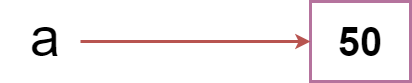
\includegraphics[width=0.7\linewidth]{img/ref1}
	\caption{Mô tả tham chiếu của biến a}
\end{figure}\par
Khi lập trình viên gán giá trị của a cho một biến b:\\
\begin{lstlisting}
a = 50
b = a
\end{lstlisting}
Biến b sẽ tham chiếu tới đối tượng mà biến a đang tham chiếu tới do Python không tạo ra đối tượng mới trong trường hợp này.
\begin{figure}[h]
	\centering
	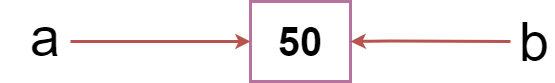
\includegraphics[width=0.7\linewidth]{img/ref2}
	\caption{Mô tả tham chiếu của biến a và b}
\end{figure}\par
Python thể hiện tính hiệu quả trong việc quản lý dữ liệu khi người lập trình gán cùng dữ liệu cho nhiều biến khác nhau.
\newpage
\subsection{Danh tính đối tượng}
Trong Python, mọi đối tượng được tạo ra đều là duy nhất. Python đảm bảo rằng không có hai đối tượng có cùng định danh. Sử dụng hàm \texttt{id()} để kiểm tra định danh của đối tượng.\par
\textbf{Ví dụ:}
\begin{lstlisting}
a = b = 1
c = 128
print(id(a))
print(id(b))
print(id(c))
\end{lstlisting}
Kết quả cho ra ở Console:
\begin{lstlisting}
1824716720
1824716720
1824718752
\end{lstlisting}
Biến a và b có cùng giá trị, do đó, chúng cùng tham chiếu đến một đối tượng nên có số \texttt{id()} như nhau. Biến c có giá trị khác a và b nên số \texttt{id()} cũng khác nhau.
\newpage
	\section{Các kiểu dữ liệu}
\subsection{Kiểu chuỗi}
Người lập trình có thể tạo ra một chuỗi bằng cách đặt nội dung vào dấu ngoặc đơn hoặc ngoặc kép.\par
\noindent
\textbf{Ví dụ:}\\
\rule{\linewidth}{0.2mm}\par
	\texttt{"Hello", 'world!'}\\
\rule{\linewidth}{0.2mm}\par
\noindent
Ngoài chuỗi trên cùng một hàng, Python hỗ trợ hai cách khởi tạo chuỗi có nội dung trên nhiều hàng:\par
\textbf{Ví dụ:}\\
\rule{\linewidth}{0.2mm}\par
\begin{linenumbers}
	\texttt{str1 = 'Hello '$\backslash$}\par
	\qquad\texttt{'World!'}\par
	\texttt{str2 = """Hello}\par
	\texttt{World!}\par
	\texttt{"""}\par
	\texttt{\textcolor{blue}{print}(str1)}\par
	\texttt{\textcolor{blue}{print}()}\par
	\texttt{\textcolor{blue}{print}(str2)}\par
\end{linenumbers}
\rule{\linewidth}{0.2mm}\par
\noindent
\resetlinenumber
Kết quả cho ra ở Console:\\
\rule{\linewidth}{0.2mm}\par
\begin{linenumbers}
	\texttt{Hello World!}\par
	\texttt{}\par
	\texttt{Hello}\par
	\texttt{World!}
\end{linenumbers}
\rule{\linewidth}{0.2mm}\par
\resetlinenumber
\newpage
\subsection{Kiểu số}
Tương tự như các ngôn ngữ lập trình khác, Python cũng có kiểu số nguyên và số thực. Ngoài ra, trong Python hỗ trợ thêm cho các lập trình viên kiểu số phức. Số nhị phân, bát phân, thập lục phân cũng được khai báo một cách dễ dàng.\par
\textbf{Ví dụ:}\\
\rule{\linewidth}{0.2mm}\par
\begin{linenumbers}
	\texttt{a = 0b10100  \# Binary Literals}\par
	\texttt{b = 100  \# Decimal Literal}\par
	\texttt{c = 0o215  \# Octal Literal}\par
	\texttt{d = 0x12d  \# Hexadecimal Literal}\par
	\texttt{f = 100.5}\par
	\texttt{z = 2 + 3j}\par
	\texttt{\textcolor{blue}{print}(a, b, c, d)}\par
	\texttt{\textcolor{blue}{print}(f)}\par
	\texttt{\textcolor{blue}{print}(z, z.real, z.imag)}\par
\end{linenumbers}
\rule{\linewidth}{0.2mm}\par
\noindent
\resetlinenumber
Kết quả cho ra ở Console:\\
\rule{\linewidth}{0.2mm}\par
\begin{linenumbers}
	\texttt{20 100 141 301}\par
	\texttt{100.5}\par
	\texttt{(2+3j) 2.0 3.0}\par
\end{linenumbers}
\rule{\linewidth}{0.2mm}\par
\resetlinenumber
\newpage
\subsection{Kiểu logic}
Kiểu logic chứa một trong hai giá trị là \texttt{True} và \texttt{False}. Trong kiểu Boolean, giá trị \texttt{True} được hiểu là 1, giá trị \texttt{False} được hiểu là 0.\par
\textbf{Ví dụ:}\\
\rule{\linewidth}{0.2mm}\par
\begin{linenumbers}
	\texttt{\textcolor{blue}{print}(\textcolor{red}{True} + 10)}\par
	\texttt{\textcolor{blue}{print}(\textcolor{red}{False} + 10)}\par
	\texttt{\textcolor{blue}{print}(\textcolor{red}{True} == 2)}\par
\end{linenumbers}
\rule{\linewidth}{0.2mm}\par
\noindent
\resetlinenumber
Kết quả cho ra ở Console:\\
\rule{\linewidth}{0.2mm}\par
\begin{linenumbers}
	\texttt{11}\par
	\texttt{10}\par
	\texttt{False}\par
\end{linenumbers}
\rule{\linewidth}{0.2mm}\par
\resetlinenumber
\newpage
\subsection{Kiểu None}
Kiểu \texttt{None} là một kiểu đặc biệt trong Python, dùng để ám chỉ một biến chưa được khởi tạo hoặc làm giá trị kết thúc của list.\par
\textbf{Ví dụ:}\\
\rule{\linewidth}{0.2mm}\par
\begin{linenumbers}
	\texttt{val1, val2 = 10, None}\par
	\texttt{\textcolor{blue}{print}(val1, val2)}\par
\end{linenumbers}
\rule{\linewidth}{0.2mm}\par
\noindent
\resetlinenumber
Kết quả cho ra ở Console:\\
\rule{\linewidth}{0.2mm}\par
\begin{linenumbers}
	\texttt{10 None}\par
\end{linenumbers}
\rule{\linewidth}{0.2mm}\par
\resetlinenumber
\newpage
\subsection{Các collections}
Python cung cấp 4 loại collection: List, Tuple, Dict và Set.
\subsubsection{List}
List có thể chứa nhiều phần tử có kiểu dữ liệu khác nhau. List có thể thay đổi, sửa đổi các phần tử bên trong được. Các giá trị trong list phân tách nhau bởi dấu phẩy và được đặt trong cặp dấu ngoặc vuông.\par
\textbf{Ví dụ:}\\
\rule{\linewidth}{0.2mm}\par
\begin{linenumbers}
	\texttt{ls = [1, 3, 5, 'Python']}\par
	\texttt{\textcolor{blue}{print}(ls)}\par
	\texttt{ls[0] = 2}\par
	\texttt{\textcolor{blue}{print}(ls)}\par
\end{linenumbers}
\rule{\linewidth}{0.2mm}\par
\noindent
\resetlinenumber
Kết quả cho ra ở Console:\\
\rule{\linewidth}{0.2mm}\par
\begin{linenumbers}
	\texttt{[1, 3, 5, 'Python']}\par
	\texttt{[2, 3, 5, 'Python']}\par
\end{linenumbers}
\rule{\linewidth}{0.2mm}\par
\resetlinenumber
\subsubsection{Tuple}
Tương tự như list, Tuple có thể chứa nhiều phần tử có kiểu dữ liệu khác nhau. Tuy nhiên, Tuple là kiểu dữ liệu immutable (không thể thay đổi các phần tử sau khi khởi tạo). Các giá trị trong Tuple phân cách nhau bởi dấu phẩy và được đặt trong cặp dấu ngoặc tròn.\par
\textbf{Ví dụ:}\\
\rule{\linewidth}{0.2mm}\par
\begin{linenumbers}
	\texttt{tpl = (1, 3, [2, "Py"])}\par
	\texttt{\textcolor{blue}{print}(tpl)}\par
	\texttt{tpl[1] = 2}\par
\end{linenumbers}
\rule{\linewidth}{0.2mm}\par
\noindent
\resetlinenumber
Kết quả cho ra ở Console:\\
\rule{\linewidth}{0.2mm}\par
\begin{linenumbers}
	\texttt{TypeError: 'tuple' object does not support item assignment}\par
	\texttt{(1, 3, [2, 'Py'])}\par
\end{linenumbers}
\rule{\linewidth}{0.2mm}\par
\resetlinenumber
\newpage
\subsubsection{Dictionary}
Dictionary lưu trữ dữ liệu bằng từng cặp key - value. Các giá trị trong Dict phân cách nhau bởi dấu phẩy và được đặt trong cặp dấu ngoặc nhọn. Cặp key - value phân cách nhau bởi dấu hai chấm.\par
\textbf{Ví dụ:}\\
\rule{\linewidth}{0.2mm}\par
\begin{linenumbers}
	\texttt{dct = \{'Name': 'An', 'Age': 21, 'School': 'ACT'\}}\par
	\texttt{\textcolor{blue}{print}(dct)}\par
\end{linenumbers}
\rule{\linewidth}{0.2mm}\par
\noindent
\resetlinenumber
Kết quả cho ra ở Console:\\
\rule{\linewidth}{0.2mm}\par
\begin{linenumbers}
	\texttt{\{'Name': 'An', 'Age': 21, 'School': 'ACT'\}}\par
\end{linenumbers}
\rule{\linewidth}{0.2mm}\par
\resetlinenumber
\subsubsection{Set}
Set lưu trữ các giá trị không theo thứ tự. Các giá trị trong Set phân cách nhau bởi dấu phẩy và được đặt trong cặp dấu ngoặc nhọn.\par
Tương tự như List và Tuple, một Set cũng có thể lưu được nhiều kiểu dữ liệu khác nhau, tuy nhiên, Set không chấp nhận phần tử có kiểu dữ liệu là List.\par
\textbf{Ví dụ:}\\
\rule{\linewidth}{0.2mm}\par
\begin{linenumbers}
	\texttt{st = \{"C++", "Java", "Python", "Scala", "Ruby", 1\}}\par
	\texttt{\textcolor{blue}{print}(st)}\par
\end{linenumbers}
\rule{\linewidth}{0.2mm}\par
\noindent
\resetlinenumber
Kết quả cho ra ở Console:\\
\rule{\linewidth}{0.2mm}\par
\begin{linenumbers}
	\texttt{\{1, 'Ruby', 'Python', 'Scala', 'C++', 'Java'\}}\par
\end{linenumbers}
\rule{\linewidth}{0.2mm}\par
\resetlinenumber
\newpage
	\section{Các từ khoá}
\label{keyword}
Từ khoá trong Python là những từ đặc biệt đối với trình biên dịch, mang một ý nghĩa nào đó. Những từ này không được dùng như tên biến.
\begin{table}[h]
	\centering
	\begin{tabular}{|l||l|}
		\hline
		Từ khoá & Ý nghĩa \\
		\hline
		\hline
		\texttt{True} & trả về giá trị \texttt{True} nếu điều kiện đưa ra là đúng. Giá trị khác 0 được hiểu là \texttt{True}. \\
		\hline
		\texttt{False} & trả về giá trị \texttt{False} nếu điều kiện đưa ra là sai. Giá trị 0 được hiểu là \texttt{False}.\\
		\hline
		\texttt{None} & biểu thị cho giá trị \texttt{null}. Một list rỗng hay giá trị 0 không được xem là \texttt{None}.\\
		\hline
		\texttt{asset} & dùng để debug trong Python, in ra lỗi của một đoạn code.\\
		\hline
		\texttt{def} & dùng để khởi tạo một hàm.\\
		\hline
		\texttt{class}& dùng để định nghĩa một lớp. Một lớp bao gồm các biến và thủ tục.\\
		\hline
		\texttt{del}& dùng để giải phóng tham chiếu tới một đối tượng.\\
		\hline
		\texttt{try, except, finally}& được dùng trong xử lý ngoại lệ. Xem mục \nameref{exception}\\
		\hline
		\texttt{raise}& tạo ngoại lệ theo định nghĩa của người lập trình. Xem mục \nameref{exception}\\
		\hline
		\texttt{and, or, not}& được sử dụng trong mệnh đề logic. Xem mục \nameref{logic}.\\
		\hline
		\texttt{for, while}& được sử dụng để tạo vòng lặp. Xem mục \nameref{for} và \nameref{while}.\\
		\hline
		\texttt{in}& kiểm tra phần tử có nằm trong một tập hợp hay không. Xem mục \nameref{kt}\\
		\hline
		\texttt{is}& xác thực phần tử. Xem mục \nameref{xt}\\
		\hline
		\texttt{if, else, elif}& được sử dụng để tạo cấu trúc rẽ nhánh. Xem mục \nameref{condition}\\
		\hline
		\texttt{continue, break, pass}& xem mục \nameref{keyloop}\\
		\hline
		\texttt{import} & dùng để thêm thư viện cho file.\\
		\hline
		\texttt{from} & dùng để thêm một hàm cụ thể trong thư viện nào đó cho file.\\
		\hline
		\texttt{as} & dùng để tạo một bí danh cho tên thư viện.\\
		\hline
		\texttt{return} & dùng để trả về một giá trị hoặc \texttt{None} trong hàm.\\
		\hline
		\texttt{gobal} & dùng để tạo một biến toàn cục.\\
		\hline
		\texttt{nonlocal} & tương tự như gobal, dùng trong các hàm lồng nhau.\\
		\hline
		\texttt{lambda} & dùng để tạo hàm vô danh.\\
		\hline
		\texttt{print} & dùng để in ra màn hình.\\
		\hline
		\texttt{input} & dùng để nhập liệu từ bàn phím.\\
		\hline
		\texttt{int} & kiểu dữ liệu integer.\\
		\hline
		\texttt{float} & kiểu dữ liệu float.\\
		\hline
	\end{tabular}
	\caption{Một số từ khoá thông dụng}
\end{table}
\newpage
	\section{Chú thích}
\subsection{Chú thích}
Chú thích trong Python là một công cụ thiết yếu cho lập trình viên, giúp giải thích, mô tả chức năng của một đoạn code nào đó.\par
Trong các ngôn ngữ lập trình khác như Java hoặc C++ cung cấp kí hiệu // cho chú thích trên một dòng và cặp kí tự /* */ cho nhiều dòng. Tuy nhiên, Python cung cấp kí hiệu \# cho chú thích trên một dòng.\par
\textbf{Ví dụ:} Hàm kiểm tra một số nguyên có phải là số nguyên tố hay không:\\
\rule{\linewidth}{0.2mm}\par
\begin{linenumbers}
	\texttt{\textcolor{red}{import} math}\par
	\smallskip
	\texttt{\textcolor{red}{def} is\_prime\_number(n):}\par
	\qquad\texttt{\# input: a integer number}\par
	\qquad\texttt{\# output: if n is a prime number, return True. If not, return False.}\par
	\smallskip
	\qquad\texttt{\# if n = 1 or n < 0, n isn't a prime number}\par
	\qquad\texttt{\textcolor{red}{if} n < 1:}\par
	\qquad\qquad\texttt{\textcolor{red}{return} False}\par
	\qquad\texttt{\# if n = 2 or n = 3, n is a prime number}\par
	\qquad\texttt{\textcolor{red}{if} n < 4:}\par
	\qquad\qquad\texttt{\textcolor{red}{return} True}\par
	\qquad\texttt{\# if n >= 4, use this function to check}\par
	\qquad\texttt{\textcolor{red}{for} i \textcolor{red}{in} range(2, int(math.sqrt(n)) + 1):}\par
	\qquad\qquad\texttt{\textcolor{red}{if} n \% i == 0:}\par
	\qquad\qquad\qquad\texttt{\textcolor{red}{return} False}\par
	\qquad\texttt{\# if n isn't multiples of i in [2, sqrt(n)], n is a prime number}\par	
	\qquad\texttt{\textcolor{red}{return} True}
\end{linenumbers}
\rule{\linewidth}{0.2mm}\par
\noindent
\resetlinenumber
\newpage
\subsection{Docstrings}
Ngoài cách chú thích sử dụng kí hiệu \#, Python hỗ trợ thêm một kiểu chú thích khác là docstrings. Docstring được dùng nhiều trong các module, hàm, lớp hoặc phương thức. Trong docstring, lập trình viên có thể mô tả chức năng của hàm, lớp, phương thức bằng cách để phần mô tả trong cặp dấu """.\par
Sử dụng hàm \texttt{\_\_doc\_\_} để in ra docstrings của một hàm. Docstrings phải được định nghĩa ở vị trí đầu tiên sau tên hàm / lớp. Nếu nằm ở vị trí khác, nó sẽ không được lưu vào hàm \texttt{\_\_doc\_\_}.\par
\textbf{Ví dụ:} Hàm in ra dòng chữ "Hello world!":\\
\rule{\linewidth}{0.2mm}\par
\begin{linenumbers}
	\texttt{\textcolor{red}{def} hello\_world():}\par
	\qquad\texttt{"""}\par
	\qquad\texttt{This function prints "Hello world!"}\par
	\qquad\texttt{"""}\par
	\qquad\texttt{\textcolor{blue}{print}("Hello world!")}\par
	\medskip
	\texttt{hello\_world()}\par
	\texttt{\textcolor{blue}{print}(hello\_world.\_\_doc\_\_)}
\end{linenumbers}
\rule{\linewidth}{0.2mm}\par
\noindent
\resetlinenumber
Kết quả cho ra ở Console:\\
\rule{\linewidth}{0.2mm}\par
\begin{linenumbers}
	\texttt{Hello world!}\par
	\texttt{}\par
	\qquad\texttt{This function prints "Hello world!"}\par
	\texttt{}
\end{linenumbers}
\rule{\linewidth}{0.2mm}
\resetlinenumber
\newpage
	\section{Toán tử}
Toán tử có thể được định nghĩa là ký hiệu chịu trách nhiệm cho một hoạt động, phép tính cụ thể giữa hai toán hạng. Python cung cấp một loạt các toán tử như sau:
\begin{itemize}
	\itemsep\setlength{0em}
	\item Toán tử số học
	\item Toán tử so sánh
	\item Toán tử gán
	\item Toán tử logic
	\item Toán tử biwter
	\item Toán tử khai thác
	\item Toán tử xác thực
\end{itemize}
\subsection{Toán tử số học}
Tương tự như Java và C, trong Python cung cấp các toán tử số học để tính toán trên các toán hạng, ngoài ra bổ sung thêm các toán tử mới.
\begin{table}[h]
	\centering
	\begin{tabular}{|l||l||l|}
		\hline
		Toán tử & Mô tả & Ví dụ \\
		\hline
		+ & Phép cộng giữa hai toán hạng & a = 10, b = 2, c = a + b (c = 12) \\
		\hline
		- & Phép trừ giữa hai toán hạng & a = 10, b = 2, c = a - b (c = 8) \\
		\hline
		* & Phép nhân giữa hai toán hạng & a = 10, b = 2, c = a * b (c = 20) \\
		\hline
		/ & Phép chia giữa hai toán hạng & a = 10, b = 2, c = a / b (c = 5)  \\
		\hline
		// & Phép chia làm tròn xuống & a = 10, b = 3, c = a // b (c = 3) \\
		\hline
		** & Phép luỹ thừa & a = 10, b = 2, c = a ** b (c = 100) \\
		\hline
		\% & Phép chia lấy dư & a = 10, b = 3, c = a \% b (c = 1) \\
		\hline
	\end{tabular}
	\caption{Mô tả các toán tử số học}
\end{table}
\subsection{Toán tử so sánh}
Toán tử so sánh dùng để so sánh giá trị của các toán hạng, kết quả trả về \texttt{True} nếu đúng và \texttt{False} nếu sai.\par
Bảng dưới đây mô tả các toán tử so sánh với a = 5, b = 2.
\begin{table}[h]
	\centering
	\begin{tabular}{|l||l||l|}
		\hline
		Toán tử & Mô tả & Ví dụ \\
		\hline
		== & So sánh bằng  & a == b (False) \\
		\hline
		!= & So sánh khác & a != b (True) \\
		\hline
		> & So sánh lớn hơn & a > b (True) \\
		\hline
		>= & So sánh lớn hơn hoặc bằng & a >= b (True) \\
		\hline
		< & So sánh bé hơn & a < b (False) \\
		\hline
		<= & So sánh bé hơn hoặc bằng & a <= b (False) \\
		\hline
	\end{tabular}
	\caption{Mô tả các toán tử so sánh}
\end{table}
\newpage
\subsection{Toán tử gán}
Toán tử gán là toán tử dùng đế gán giá trị của một đối tượng cho một đối tượng khác. Trong Python, nó cũng được thể hiện giống như các ngôn ngữ khác.\par
Bảng dưới đây mô tả các toán tử gán với a = 5, b = 2.
\begin{table}[h]
	\centering
	\begin{tabular}{|l||l||l|}
		\hline
		Toán tử & Mô tả & Ví dụ \\
		\hline
		= & Gán giá trị của toán hạng này cho toán hạng khác & a = b (a = 2) \\
		\hline
		+= & Cộng toán hạng này cho toán hạng kia rồi gán lại cho chính nó & a += b (a = 7) \\
		\hline
		-= & Trừ toán hạng này cho toán hạng kia rồi gán lại cho chính nó & a -= b (a = 3) \\
		\hline
		*= & Nhân toán hạng này cho toán hạng kia rồi gán lại cho chính nó & a *= b (a = 10) \\
		\hline
		/= & Chia toán hạng này cho toán hạng kia rồi gán lại cho chính nó & a /= b (a = 2.5) \\
		\hline
		\%= & Chia lấy dư toán hạng này cho toán hạng kia rồi gán lại cho chính nó & a \%= b (a = 1) \\
		\hline
		**= & Luỹ thừa toán hạng này cho toán hạng kia rồi gán lại cho chính nó & a **= b (a = 25) \\
		\hline
		//= & Chia làm tròn xuống toán hạng này cho toán hạng kia rồi gán lại cho chính nó & a //= b (a = 2) \\
		\hline
	\end{tabular}
	\caption{Mô tả các toán tử gán}
\end{table}
\subsection{Toán tử logic}
\label{logic}
Tương tự các ngôn ngữ khác, trong Python có 3 loại toán tử logic: \texttt{and}, \texttt{or}, \texttt{not}.\par
Bảng dưới đây mô tả các toán tử logic trong Python, với a = \texttt{True}, b = \texttt{False}.
\begin{table}[h]
	\centering
	\begin{tabular}{|l||l||l|}
		\hline
		Toán tử & Mô tả & Ví dụ \\
		\hline
		and & Nếu cả hai vế của toán tử đều là True thì kết quả là True, ngược lại là False & a and b (False) \\
		\hline
		or  & Nếu một trong hai vế của toán tử là True thì kết quả là True, ngược lại là False & a or b (True) \\
		\hline
		not & Nếu toán tử là True thì kết quả là False, ngược lại là True & not a (False) \\
		\hline
	\end{tabular}
	\caption{Mô tả các toán tử logic}
\end{table}
\subsection{Toán tử biwter}
Toán tử biwter thực hiện trên các bit nhị phân của các giá trị.\par
Bảng dưới đây mô tả các toán tử biwter trong Python, với a = 00001100, b = 00001111.
\begin{table}[h]
	\centering
	\begin{tabular}{|l||l|}
		\hline
		Toán tử & Ví dụ \\
		\hline
		| & (a | b) (00001111) \\
		\hline
		\& & (a \& b) (00001100) \\
		\hline
		\^{} & (a \^{} b) (00000010)  \\
		\hline
		\~{} & (\~{}a) = (00001101) \\
		\hline
		<< & a<<a  (49152) \\
		\hline
		>> & a>>a (0) \\
		\hline
	\end{tabular}
	\caption{Mô tả các toán tử biwter}
\end{table}
\newpage
\subsection{Toán tử khai thác}
\label{kt}
Toán tử khai thác thường được dùng để kiểm tra xem 1 đối số có nằm trong 1 tập hợp đối số hay không. Trong Python hỗ trợ hai dạng toán tử khai thác là \texttt{in} và \texttt{not in}.\par
Bảng dưới đây mô tả các toán tử khai thác trong Python với a = 6, b = [1, 6, 5].
\begin{table}[h]
	\centering
	\begin{tabular}{|l||l||l|}
		\hline
		Toán tử & Mô tả & Ví dụ \\
		\hline
		in  & Kiểm tra đối số có nẳm trong tập hợp không & a in b (True) \\
		\hline
		not in & Kiểm tra đối số có nẳm ngoài tập hợp không & a not in b (False) \\
		\hline
	\end{tabular}
	\caption{Mô tả các toán tử khai thác}
\end{table}
\subsection{Toán tử xác thực}
\label{xt}
Toán tử xác thực dùng để kiểm hai giá trị có bằng nhau hay không. Trong Python hỗ trợ 2 dạng toán tử xác thực là \texttt{is} và \texttt{not is}.\par
Bảng dưới đây mô tả các toán tử xác thực trong Python với a = 6, b = 7.
\begin{table}[h]
	\centering
	\begin{tabular}{|l||l||l|}
		\hline
		Toán tử & Mô tả & Ví dụ \\
		\hline
		is  & Kiểm tra toán hạng này có bằng toán hạng kia hay không & a is b (False) \\
		\hline
		not is & Kiểm tra toán hạng này có khác toán hạng kia hay không & a not is b (True) \\
		\hline
	\end{tabular}
	\caption{Mô tả các toán tử xác thực}
\end{table}
\newpage
	\section{Nhập, xuất dữ liệu}
Sử dụng lệnh \texttt{print(<string>)} để in chuỗi ra ngoài màn hình.\par
\textbf{Ví dụ:} Chương trình Hello World!\\
\rule{\linewidth}{0.2mm}\par
\begin{linenumbers}
	\texttt{\textcolor{blue}{print}("Hello World!")}
\end{linenumbers}
\rule{\linewidth}{0.2mm}\par
\noindent
\resetlinenumber
Kết quả cho ra ở Console:\\
\rule{\linewidth}{0.2mm}\par
\begin{linenumbers}
	\texttt{Hello World!}
\end{linenumbers}
\rule{\linewidth}{0.2mm}
\resetlinenumber
\newpage
Sử dụng hàm \texttt{input()} để đưa dữ liệu từ bàn phím vào trong Python, cú pháp:
\begin{center}
	\texttt{<variable\_name> = input([<output\_string>])}
\end{center}
\textbf{Ví dụ:} Chương trình nhập vào tên người dùng, in ra kết quả \texttt{“Hello + tên người dùng”}:\\
\rule{\linewidth}{0.2mm}\par
\begin{linenumbers}
	\texttt{userName = \textcolor{blue}{input}("Type your name here: ")}\par
	\texttt{\textcolor{blue}{print}("Hello " + userName)}
\end{linenumbers}
\rule{\linewidth}{0.2mm}\par
\noindent
\resetlinenumber
Kết quả cho ra ở Console:\\
\rule{\linewidth}{0.2mm}\par
\begin{linenumbers}
	\texttt{Type your name here: An}\par
	\texttt{Hello An}
\end{linenumbers}
\rule{\linewidth}{0.2mm}\par
\resetlinenumber
\newpage
Mặc định dữ liệu đưa vào khi sử dụng hàm \texttt{input()} là một chuỗi:\\
\rule{\linewidth}{0.2mm}\par
\begin{linenumbers}
	\texttt{a = \textcolor{blue}{input}("a = ")}\par
	\texttt{b = \textcolor{blue}{input}("b = ")}\par
	\texttt{\textcolor{blue}{print}('a is',type(a), 'format')}\par
	\texttt{\textcolor{blue}{print}('b is',type(b), 'format')}\par
	\texttt{c = a + b}\par
	\texttt{\textcolor{blue}{print}('a + b = ', c)}\par
\end{linenumbers}
\rule{\linewidth}{0.2mm}\par
\noindent
\resetlinenumber
Kết quả cho ra ở Console:\\
\rule{\linewidth}{0.2mm}\par
\begin{linenumbers}
	\texttt{a = 15}\par
	\texttt{b = 36}\par
	\texttt{a is <class 'str'> format}\par
	\texttt{b is <class 'str'> format}\par
	\texttt{a + b =  1536}
\end{linenumbers}
\rule{\linewidth}{0.2mm}\par
\resetlinenumber
Khi nhập vào một số, để thuận tiện cho việc tính toán, ta phải ép kiểu chuỗi về số.\par
\noindent
\textbf{Ví dụ:} Chương trình nhập vào năm sinh người dùng, trả về tuổi của người đó tính đến năm 2020:\\
\rule{\linewidth}{0.2mm}\par
\begin{linenumbers}
	\texttt{year = \textcolor{red}{int}(\textcolor{blue}{print}("Type your year of birth here: "))}\par
	\texttt{age = 2020 - year}\par
	\texttt{\textcolor{blue}{print}("Your age is: \%d" \% age)}
\end{linenumbers}
\rule{\linewidth}{0.2mm}\par
\noindent
\resetlinenumber
Kết quả cho ra ở Console:\\
\rule{\linewidth}{0.2mm}\par
\begin{linenumbers}
	\texttt{Type your year of birth here: 1999}\par
	\texttt{Your age is: 21}
\end{linenumbers}
\rule{\linewidth}{0.2mm}\par
\resetlinenumber
\newpage
	\section{Câu lệnh rẽ nhánh}
\label{condition}
Câu lệnh rẽ nhánh là câu lệnh quen thuộc và được sử dụng rất nhiều trong các ngôn ngữ lập trình. Câu lệnh này kiểm tra một điều kiện vào, xử lý dữ liệu với từng trường hợp đúng sai của điều kiện đó.\par
Trong Python, mọi giá trị \texttt{<condition>} khác 0 và None được hiểu là \texttt{true}.
\subsection{Câu lệnh if}
Câu lệnh if dùng để kiểm tra một điều kiện với đầu vào là một mệnh đề logic. Nếu điều kiện đúng sẽ thực hiện câu lệnh, nếu sai thì câu lệnh sẽ không được thực hiện.\par
Cấu trúc của câu lệnh if:\par
\texttt{if <condition>:}\par
\qquad \texttt{//conditional code}\par
\begin{figure}[h]
	\centering
	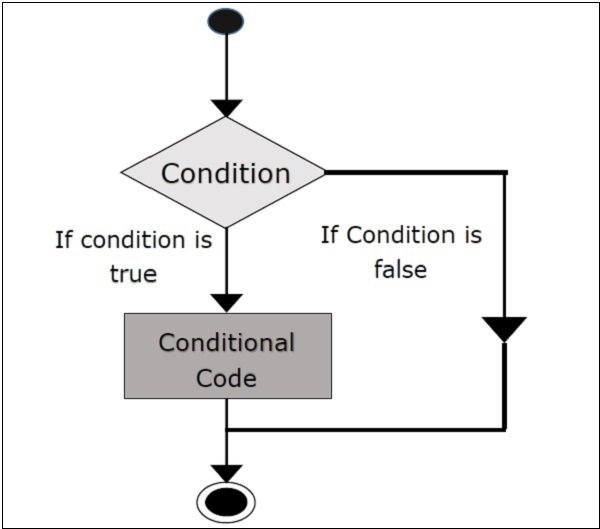
\includegraphics[width=0.7\linewidth]{img/if}
	\caption{Mô tả cách thức hoạt động của câu lệnh if}
\end{figure}
\newpage
\textbf{Ví dụ:} Chương trình nhập vào một số nguyên, nếu số đó là số chẵn thì in ra màn hình:\\
\rule{\linewidth}{0.2mm}\par
\begin{linenumbers}
	\texttt{number = \textcolor{red}{int}(\textcolor{blue}{input}("Type a number: "))}\par
	\texttt{\textcolor{red}{if} number \% 2 == 0:}\par
	\qquad \texttt{\textcolor{blue}{print}("\%d is an even number." \% number)}
\end{linenumbers}
\rule{\linewidth}{0.2mm}\par
\noindent
\resetlinenumber
Kết quả cho ra ở Console:\\
\rule{\linewidth}{0.2mm}\par
\begin{linenumbers}
	\texttt{Type a number: 12}\par
	\texttt{12 is an even number.}
\end{linenumbers}
\rule{\linewidth}{0.2mm}\par
\resetlinenumber
\newpage
\textbf{Ví dụ:}  Kiểm tra tuổi của sinh viên, nếu trên 17 là được chấp nhận:\\
\rule{\linewidth}{0.2mm}\par
\begin{linenumbers}
	\texttt{age = \textcolor{red}{int}(\textcolor{blue}{input}("Type your age: "))}\par
	\texttt{\textcolor{red}{if} age > 17: }\par
	\qquad \texttt{\textcolor{blue}{print}("Accepted!")}
\end{linenumbers}
\rule{\linewidth}{0.2mm}\par
\noindent
\resetlinenumber
Kết quả cho ra ở Console:\\
\rule{\linewidth}{0.2mm}\par
\begin{linenumbers}
	\texttt{Type your age: 16}\par
\end{linenumbers}
\rule{\linewidth}{0.2mm}\par
\resetlinenumber
\newpage
\subsection{Câu lệnh if - else}
Ở câu lệnh if, chương trình chỉ thực thi khối lệnh nếu điều kiện vào là đúng. Trong nhiều trường hợp, ta cũng cần phải xử lý chương trình khi điều kiện vào là sai. Việc sử dụng từ khoá \texttt{else} sẽ giải quyết được trường hợp trên.\par
Cấu trúc của câu lệnh if - else:\par
\texttt{if <condition>:}\par
\qquad \texttt{//if block's code}\par
\texttt{else:}\par
\qquad \texttt{//else block's code}\par
\begin{figure}[h]
	\centering
	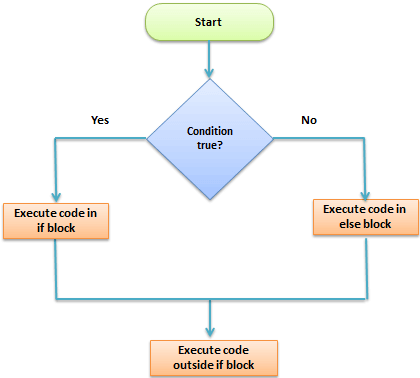
\includegraphics{img/if_else}
	\caption{Mô tả cách thức hoạt động của câu lệnh if - else}
\end{figure}
\newpage
\textbf{Ví dụ:} Chương trình nhập vào một số nguyên, kiểm tra đó là số chẵn hay lẻ:\\
\rule{\linewidth}{0.2mm}\par
\begin{linenumbers}
	\texttt{number = \textcolor{red}{int}(\textcolor{blue}{input}("Type a number: "))}\par
	\texttt{\textcolor{red}{if} number \% 2 == 0:}\par
	\qquad \texttt{\textcolor{blue}{print}("\%d is an even number." \% number)}\par
	\texttt{\textcolor{red}{else}:}\par
	\qquad \texttt{\textcolor{blue}{print}("\%d is an odd number." \% number)}\par
\end{linenumbers}
\rule{\linewidth}{0.2mm}\par
\noindent
\resetlinenumber
Kết quả cho ra ở Console:\\
\rule{\linewidth}{0.2mm}\par
\begin{linenumbers}
	\texttt{Type a number: 11}\par
	\texttt{11 is an odd number.}
\end{linenumbers}
\rule{\linewidth}{0.2mm}\par
\resetlinenumber
\newpage
\textbf{Ví dụ:} Chương trình xếp loại, với điểm >= 8 xếp loại giỏi, >= 7 xếp loại khá và còn lại là trung bình:\\
\rule{\linewidth}{0.2mm}\par
\begin{linenumbers}
	\texttt{score = \textcolor{red}{float}(\textcolor{blue}{input}("Type your score: "))}\par
	\texttt{\textcolor{red}{if} score >= 8:}\par
	\qquad \texttt{\textcolor{blue}{print}("Excellent")}\par
	\texttt{\textcolor{red}{else}:}\par
	\qquad \texttt{\textcolor{red}{if} score >= 7:}\par
	\qquad \qquad \texttt{\textcolor{blue}{print}("Good")}\par
	\qquad \texttt{\textcolor{red}{else}:}\par
	\qquad \qquad \texttt{\textcolor{blue}{print}("Medium")}\par
\end{linenumbers}
\rule{\linewidth}{0.2mm}\par
\noindent
\resetlinenumber
Kết quả cho ra ở Console:\\
\rule{\linewidth}{0.2mm}\par
\begin{linenumbers}
	\texttt{Type your score: 6.2}\par
	\texttt{Medium}
\end{linenumbers}
\rule{\linewidth}{0.2mm}\par
\resetlinenumber
\newpage
\subsection{Câu lệnh if - elif (else if) - else}
Trong trường hợp cần xét nhiều hơn 2 điều kiện, thay vì sử dụng \texttt{else: if <condition>:}, ta có thể viết gọn thành \texttt{elif}.\par
Cấu trúc của câu lệnh if - elif - else:\par
\texttt{if <condition>:}\par
\qquad \texttt{//if block's code}\par
\texttt{elif <condition>:}\par
\qquad \texttt{//elif block's code}\par
\texttt{[elif <condition>:}\par
\qquad \texttt{//elif block's code]}\par
\texttt{[...]}\par
\texttt{else:}\par
\qquad \texttt{//else block's code}\par
\begin{figure}[h]
	\centering
	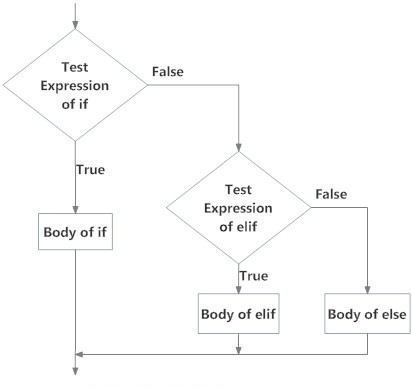
\includegraphics{img/if_elif}
	\caption{Mô tả cách thức hoạt động của câu lệnh if - elif - else}
\end{figure}
\newpage
\textbf{Ví dụ:} Chương trình nhập vào một số, kiểm tra số đó là số âm, số dương hay số 0:\\
\rule{\linewidth}{0.2mm}\par
\begin{linenumbers}
	\texttt{number = \textcolor{red}{float}(\textcolor{blue}{input}("Type a number: "))}\par
	\texttt{\textcolor{red}{if} number > 0:}\par
	\qquad \texttt{\textcolor{blue}{print}("\%.3f is a positive number." \% number)}\par
	\texttt{\textcolor{red}{elif} number < 0:}\par
	\qquad \texttt{\textcolor{blue}{print}("\%.3f is a negative number." \% number)}\par
	\texttt{\textcolor{red}{else}:}\par
	\qquad \texttt{\textcolor{blue}{print}("The number is 0.")}\par
\end{linenumbers}
\rule{\linewidth}{0.2mm}\par
\noindent
\resetlinenumber
Kết quả cho ra ở Console:\\
\rule{\linewidth}{0.2mm}\par
\begin{linenumbers}
	\texttt{Type a number: -18.25}\par
	\texttt{-18.250 is a negative number.}
\end{linenumbers}
\rule{\linewidth}{0.2mm}\par
\resetlinenumber
\newpage
\textbf{Ví dụ:} Chương trình giải phương trình bậc 2:\\
\rule{\linewidth}{0.2mm}\par
\begin{linenumbers}
	\texttt{\textcolor{red}{import} math}\par
	\bigskip
	\texttt{a = \textcolor{red}{int}(\textcolor{blue}{input}("Type your first coefficient: "))}\par
	\texttt{b = \textcolor{red}{int}(\textcolor{blue}{input}("Type your second coefficient: "))}\par
	\texttt{c = \textcolor{red}{int}(\textcolor{blue}{input}("Type your third coefficient: "))}\par
	\texttt{delta = b * b - 4 * a * c}\par
	\texttt{\textcolor{red}{if} delta < 0:}\par
	\qquad \texttt{\textcolor{blue}{print}("The equation has no solution.")}\par
	\texttt{\textcolor{red}{elif} delta == 0:}\par
	\qquad \texttt{x = - b / (2 * a)}\par
	\qquad \texttt{\textcolor{blue}{print}("x = \%.2f" \% x)}\par
	\texttt{\textcolor{red}{else}:}\par
	\qquad \texttt{x1 = (-b - math.sqrt(delta)) / (2 * a)}\par
	\qquad \texttt{x2 = (-b + math.sqrt(delta)) / (2 * a)}\par
	\qquad \texttt{\textcolor{blue}{print}("x1 = \%.2f, x2 = \%.2f" \% (x1, x2))}\par
\end{linenumbers}
\rule{\linewidth}{0.2mm}\par
\noindent
\resetlinenumber
Kết quả cho ra ở Console với ví dụ giải phương trình $2x^2 + 3x - 1$:\\
\rule{\linewidth}{0.2mm}\par
\begin{linenumbers}
	\texttt{Type your first coefficient: 2}\par
	\texttt{Type your second coefficient: 3}\par
	\texttt{Type your third coefficient: 1}\par
	\texttt{x1 = -1.00, x2 = -0.50}
\end{linenumbers}
\rule{\linewidth}{0.2mm}\par
\resetlinenumber
\newpage
\textbf{Ví dụ:} Chương trình giải hệ phương trình bậc nhất hai ẩn:\\
\rule{\linewidth}{0.2mm}\par
\begin{linenumbers}
	\texttt{a1 = \textcolor{red}{int}(\textcolor{blue}{input}("a1 = "))}\par
	\texttt{b1 = \textcolor{red}{int}(\textcolor{blue}{input}("b1 = "))}\par
	\texttt{c1 = \textcolor{red}{int}(\textcolor{blue}{input}("c1 = "))}\par
	\medskip
	\texttt{a2 = \textcolor{red}{int}(\textcolor{blue}{input}("a2 = "))}\par
	\texttt{b2 = \textcolor{red}{int}(\textcolor{blue}{input}("b2 = "))}\par
	\texttt{c2 = \textcolor{red}{int}(\textcolor{blue}{input}("c2 = "))}\par
	\medskip
	\texttt{d = a1 * b2 - a2 * b1}\par
	\texttt{dx = c1 * b2 - c2 * b1}\par
	\texttt{dy = a1 * c2 - a2 * c1}\par
	\medskip
	\texttt{\textcolor{red}{if} d == 0 and dx == dy and dx == 0:}\par
	\qquad \texttt{\textcolor{blue}{print}("This equations has an infinite number of solutions.")}\par
	\texttt{\textcolor{red}{elif} d == 0 and dx != dy:}\par
	\qquad \texttt{\textcolor{blue}{print}("This equations has no solution.")}\par
	\texttt{\textcolor{red}{else}:}\par
	\qquad \texttt{x = dx / d}\par
	\qquad \texttt{y = dy / d}\par
	\qquad \texttt{\textcolor{blue}{print}("x = \%.2f, y = \%.2f" \% (x, y))}\par
\end{linenumbers}
\rule{\linewidth}{0.2mm}\par
\noindent
\resetlinenumber
Kết quả cho ra ở Console với ví dụ giải hệ phương trình
$\begin{cases}
	x - y = 1\\
	x + y = 3
\end{cases}$:\par
\noindent
\rule{\linewidth}{0.2mm}\par
\begin{linenumbers}
	\texttt{a1 = 1}\par
	\texttt{b1 = -1}\par
	\texttt{c1 = 1}\par
	\texttt{a2 = 1}\par
	\texttt{b2 = 1}\par
	\texttt{c2 = 3}\par
	\texttt{x = 2.00, y = 1.00}
\end{linenumbers}
\rule{\linewidth}{0.2mm}\par
\resetlinenumber
\newpage
\subsection{Switch - case}
Python không có cấu trúc switch case đơn giản. Thay vào đó, chúng ta có thể sử dụng một dictionary để ánh xạ đến các case.\par
Cấu trúc một dictionary:\par
\texttt{<name of dictionary> = \{}\par
\qquad \texttt{<key 1>: <value 1>,}\par
\qquad \texttt{[<key 2>: <value 2>,]}\par
\qquad \texttt{[<key 3>: <value 3>,]}\par
\qquad \texttt{[...]}\par
\texttt{\}}\par
Ta sử dụng hàm \texttt{get(<key>, <value if key not found>)} để lấy value từ một key đã biết trước.
\newpage
\textbf{Ví dụ:} Chương trình nhập vào tháng dạng số nguyên, xuất ra tên tháng:\\
\rule{\linewidth}{0.2mm}\par
\begin{linenumbers}
	\texttt{\textcolor{red}{def} get\_month\_by\_number(month):}\par
	\qquad \texttt{switch = \{}\par
	\qquad \qquad \texttt{1: 'January',}\par
	\qquad \qquad \texttt{2: 'February',}\par
	\qquad \qquad \texttt{3: 'March',}\par
	\qquad \qquad \texttt{4: 'April',}\par
	\qquad \qquad \texttt{5: 'May',}\par
	\qquad \qquad \texttt{6: 'June',}\par
	\qquad \qquad \texttt{7: 'July',}\par
	\qquad \qquad \texttt{8: 'August',}\par
	\qquad \qquad \texttt{9: 'September',}\par
	\qquad \qquad \texttt{10: 'October',}\par
	\qquad \qquad \texttt{11: 'November',}\par
	\qquad \qquad \texttt{12: 'December'}\par
	\qquad \texttt{\}}\par
	\qquad \texttt{\textcolor{red}{return}  switch.get(month, 'Month must be less than 13 and greater than 0.')}\par
	\bigskip
	\texttt{month = \textcolor{red}{int}(\textcolor{blue}{input}("Type your month: "))}\par
	\texttt{\textcolor{blue}{print}(get\_month\_by\_number(month))}\par
\end{linenumbers}
\rule{\linewidth}{0.2mm}\par
\noindent
\resetlinenumber
Kết quả cho ra ở Console:\\
\rule{\linewidth}{0.2mm}\par
\begin{linenumbers}
	\texttt{Type your month: 8}\par
	\texttt{August}\par
\end{linenumbers}
\rule{\linewidth}{0.2mm}\par
\resetlinenumber
\newpage
\textbf{Ví dụ:} Chương trình nhập vào tháng dạng số nguyên, xuất số ngày trong tháng:\\
\rule{\linewidth}{0.2mm}\par
\begin{linenumbers}
	\texttt{\textcolor{red}{def} get\_month\_by\_number(month):}\par
	\qquad \texttt{switch = \{}\par
	\qquad \qquad \texttt{1: 'January', 2: 'February', 3: 'March', 4: 'April', }\par
	\qquad \qquad \texttt{5: 'May', 6: 'June', 7: 'July', 8: 'August', }\par
	\qquad \qquad \texttt{9: 'September', 10: 'October', 11: 'November', 12: 'December'}\par
	\qquad \texttt{\}}\par
	\medskip
	\texttt{\textcolor{red}{def} get\_day\_of\_february():}\par
	\qquad \texttt{year = \textcolor{red}{int}(\textcolor{blue}{input}("Type a year: "))}\par
	\qquad \texttt{\textcolor{red}{if} year \% 400 == 0 or (year \% 4 == 0 and year \% 100 != 0):}\par
	\qquad \qquad \texttt{return 29}\par
	\qquad \texttt{return 28}\par
	\medskip
	\texttt{\textcolor{red}{def} get\_day\_of\_month(month):}\par
	\qquad \texttt{switch = \{}\par
	\qquad \qquad \texttt{1: 31, 2: get\_day\_of\_february(),}\par
	\qquad \qquad \texttt{3: 31, 4: 30,}\par
	\qquad \qquad \texttt{5: 31, 6: 30,}\par
	\qquad \qquad \texttt{7: 31, 8: 31,}\par
	\qquad \qquad \texttt{9: 30, 10: 31,}\par
	\qquad \qquad \texttt{11: 30, 12: 31}\par
	\qquad \texttt{\}}\par
	\qquad \texttt{\textcolor{red}{return}  switch.get(month, 'Month must be less than 13 and greater than 0.')}\par
	\medskip
	\texttt{month = \textcolor{red}{int}(\textcolor{blue}{input}("Type a month: "))}\par
	\texttt{\textcolor{blue}{print}(get\_month\_by\_number(month), 'has', get\_day\_of\_month(month), 'days.')}\par
\end{linenumbers}
\rule{\linewidth}{0.2mm}\par
\noindent
\resetlinenumber
Kết quả cho ra ở Console:\\
\rule{\linewidth}{0.2mm}\par
\begin{linenumbers}
	\texttt{Type a month: 2}\par
	\texttt{Type a year: 2003}\par
	\texttt{February has 28 days.}\par
\end{linenumbers}
\rule{\linewidth}{0.2mm}\par
\resetlinenumber
\newpage




\newpage
	\section{Vòng lặp}
Sử dụng vòng lặp khi ta muốn lặp đi lặp lại một đoạn code nhiều lần. Có hai loại vòng lặp:
\begin{itemize}
	\itemsep\setlength{0em}
	\item Vòng lặp xác định (definite loop): việc lặp sẽ được thực hiện với số lần biết trước.
	\item Vòng lặp không xác định (indefinite loop): việc lặp sẽ được thực hiện với số lần không biết trước.
\end{itemize}
\newpage
\subsection{Vòng lặp for}
\label{for}
Sử dụng vòng lặp for để lặp đi lặp loại một khối lệnh khi biết số lần lặp cụ thể. Cấu trúc vòng lặp for:\par
\texttt{for <iterator\_var> in <sequence>:}\par
	\qquad // \texttt{for block's code}\par
Trong đó:
\begin{itemize}
	\itemsep\setlength{0em}
	\item \texttt{sequence} là chuỗi hoặc collection ... cần lặp.
	\item \texttt{iterator\_var} là biến lặp, nhận giá trị của từng phần tử bên trong \texttt{sequence} ở mỗi lần lặp.
\end{itemize}
\begin{figure}[h]
	\centering
	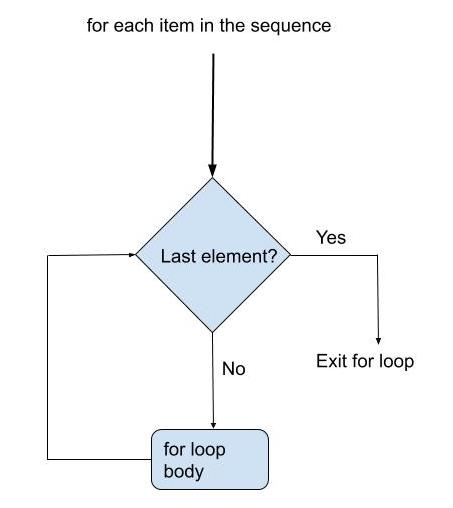
\includegraphics[width=0.5\linewidth]{img/for}
	\caption{Mô tả cách thức hoạt động của vòng lặp for}
\end{figure}
Do vòng lặp for của Python chỉ duyệt qua các phần tử có trong \texttt{sequence} nên đối với các bài toán không thao tác trên chuỗi hoặc các collections, ta phải dùng thêm hàm \texttt{range()} để trả về một danh sách các số~hạng theo thứ tự cần lặp.
\begin{table}[h]
	\centering
	\begin{tabular}{|l||l||l||l|}
		\hline
		Cấu trúc  & Giá trị & Ví dụ & Kết quả \\
		\hline
		range(n) & [0, 1, 2,... n - 1] & range(3) & [0, 1, 2] \\
		\hline
		range(x, y) & [x, x + 1, x + 2,... y - 1] & range(2, 5) & [2, 3, 4] \\
		\hline
		range(x, y, n) & [x, x + n, x + 2n,.... y'] (y' <= y - 1) & range(3, 8, 2) & [3, 5, 7] \\
		\hline
	\end{tabular}
	\caption{Mô tả kết quả hàm range()}
\end{table}
\newpage
\textbf{Ví dụ:} Chương trình nhập vào một số, tính giai thừa của số đó:\\
\rule{\linewidth}{0.2mm}\par
\begin{linenumbers}
	\texttt{n = \textcolor{red}{int}(\textcolor{blue}{input}("Type a number: "))}\par
	\texttt{factorial = 1}\par
	\texttt{\textcolor{red}{for} i \textcolor{red}{in} range(2, n + 1):}\par
	\qquad \texttt{factorial *= i}\par
	\texttt{\textcolor{blue}{print}("Factorial of \%d: \%d" \% (n, factorial))}\par
\end{linenumbers}
\rule{\linewidth}{0.2mm}\par
\noindent
\resetlinenumber
Kết quả cho ra ở Console:\\
\rule{\linewidth}{0.2mm}\par
\begin{linenumbers}
	\texttt{Type a number: 6}\par
	\texttt{Factorial of 6: 720}\par
\end{linenumbers}
\rule{\linewidth}{0.2mm}\par
\resetlinenumber
\newpage
\textbf{Ví dụ:} Chương trình nhập vào một số, tính tổng số chẵn trong đoạn [2, n]:\\
\rule{\linewidth}{0.2mm}\par
\begin{linenumbers}
	\texttt{n = \textcolor{red}{int}(\textcolor{blue}{input}("Type a number: "))}\par
	\texttt{sum = 0}\par
	\texttt{\textcolor{red}{for} i \textcolor{red}{in} range(2, n + 1, 2):}\par
	\qquad \texttt{sum += i}\par
	\texttt{\textcolor{blue}{print}("Sum of even numbers in [2, \%d]: \%d" \% (n, sum))}\par
\end{linenumbers}
\rule{\linewidth}{0.2mm}\par
\noindent
\resetlinenumber
Kết quả cho ra ở Console:\\
\rule{\linewidth}{0.2mm}\par
\begin{linenumbers}
	\texttt{Type a number: 6}\par
	\texttt{Sum of even numbers in [2, 6]: 12}\par
\end{linenumbers}
\rule{\linewidth}{0.2mm}\par
\resetlinenumber
\newpage
\textbf{Ví dụ:} Chương trình nhập vào một chuỗi, in ra từng ký tự trong chuỗi:\\
\rule{\linewidth}{0.2mm}\par
\begin{linenumbers}
	\texttt{string = \textcolor{blue}{input}("Type a sentence: ")}\par
	\texttt{\textcolor{red}{for} char \textcolor{red}{in} string:}\par
	\qquad \texttt{\textcolor{blue}{print}(char)}\par
\end{linenumbers}
\rule{\linewidth}{0.2mm}\par
\noindent
\resetlinenumber
Kết quả cho ra ở Console:\\
\rule{\linewidth}{0.2mm}\par
\begin{linenumbers}
	\texttt{Type a sentence: Python}\par
	\texttt{P}\par
	\texttt{y}\par
	\texttt{t}\par
	\texttt{t}\par
	\texttt{o}\par
	\texttt{n}\par
\end{linenumbers}
\rule{\linewidth}{0.2mm}\par
\resetlinenumber
\newpage
\textbf{Ví dụ:} Chương trình tính tổng, tích một dãy số sử dụng vòng lặp for duyệt qua các phần tử trong mảng:\\
\rule{\linewidth}{0.2mm}\par
\begin{linenumbers}
	\texttt{array = [1, 3, 5, 8, 9]}\par
	\texttt{sum = 0}\par
	\texttt{product = 1}\par
	\texttt{\textcolor{red}{for} element \textcolor{red}{in} array:}\par
	\qquad \texttt{sum += element}\par
	\qquad \texttt{product *= element}\par
	\texttt{\textcolor{blue}{print}("Sum of array: ", sum)}\par
	\texttt{\textcolor{blue}{print}("Product of array: ", product)}
\end{linenumbers}
\rule{\linewidth}{0.2mm}\par
\noindent
\resetlinenumber
Kết quả cho ra ở Console:\\
\rule{\linewidth}{0.2mm}\par
\begin{linenumbers}
	\texttt{Sum of array:  26}\par
	\texttt{Produce of array:  1080}\par
\end{linenumbers}
\rule{\linewidth}{0.2mm}\par
\resetlinenumber
\newpage
Chúng ta cũng có thể duyệt mảng bằng các sử dụng chỉ số của từng phần tử. Sử dụng hàm \texttt{len(obj)} để trả về độ dài của mảng.\par
\noindent
\textbf{Ví dụ:} Chương trình nhập vào một dãy số, tính tổng các số lẻ trong dãy:\\
\rule{\linewidth}{0.2mm}\par
\begin{linenumbers}
	\texttt{length = \textcolor{red}{int}(\textcolor{blue}{input}("Type length of array: "))}\par
	\texttt{array = []}\par
	\texttt{sum = 0}\par
	\texttt{\textcolor{red}{for} i \textcolor{red}{in} range(length):}\par
	\qquad \texttt{array.append(\textcolor{red}{int}(\textcolor{blue}{input}("Type your number \%d: " \% (i + 1))))}\par
	\texttt{\textcolor{blue}{print}("Iterating over array by index:")}\par
	\texttt{\textcolor{red}{for} i \textcolor{red}{in} range(len(array)):}\par
	\qquad \texttt{\textcolor{blue}{print}("Index \%d: \%d" \%(i, array[i]))}\par
	\qquad \texttt{\textcolor{red}{if} array[i] \% 2 == 1:}\par
	\qquad \qquad \texttt{sum += array[i]}\par
	\texttt{\textcolor{blue}{print}("Sum of odd numbers in array: ", sum)}\par
\end{linenumbers}
\rule{\linewidth}{0.2mm}\par
\noindent
\resetlinenumber
Kết quả cho ra ở Console:\\
\rule{\linewidth}{0.2mm}\par
\begin{linenumbers}
	\texttt{Type length of array: 3}\par
	\texttt{Type your number 1: 1}\par
	\texttt{Type your number 2: 4}\par
	\texttt{Type your number 3: 9}\par
	\texttt{Iterating over array by index:}\par
	\texttt{Index 0: 1}\par
	\texttt{Index 1: 4}\par
	\texttt{Index 2: 9}\par
	\texttt{Sum of odd numbers in array:  10}
\end{linenumbers}
\rule{\linewidth}{0.2mm}\par
\resetlinenumber
\newpage
\subsection{Vòng lặp while}
\label{while}
Sử dụng vòng lặp while để lặp đi lặp loại một khối lệnh khi số lần lặp phụ thuộc vào điều kiện lặp. Cấu trúc của vòng lặp while:\par
\texttt{while <condition>:}\par
\qquad \texttt{//while block's code}\par
\texttt{[else:}\par
\qquad \texttt{//else block's code]}\par
\begin{figure}[h]
	\centering
	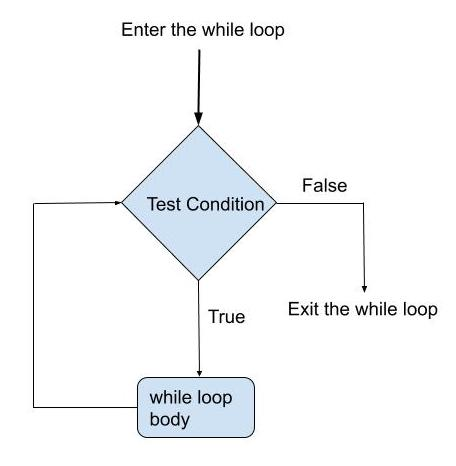
\includegraphics[width=0.5\linewidth]{img/while}
	\caption{Mô tả cách thức hoạt động của vòng lặp while}
	\label{fig:while}
\end{figure}
\newpage
\textbf{Ví dụ:} Chương trình nhập vào một số, in ra các bội nhỏ hơn 100 của số đó :\\
\rule{\linewidth}{0.2mm}\par
\begin{linenumbers}
	\texttt{n = \textcolor{red}{int}(\textcolor{blue}{input}("Type a number: "))}\par
	\texttt{multiple = n}\par
	\texttt{i = 2}\par
	\texttt{\textcolor{red}{while} multiple < 100:}\par
	\qquad \texttt{\textcolor{blue}{print}(multiple)}\par
	\qquad\texttt{multiple = n}\par
	\qquad\texttt{multiple *= i}\par
	\qquad\texttt{i += 1}\par
\end{linenumbers}
\rule{\linewidth}{0.2mm}\par
\noindent
\resetlinenumber
Kết quả cho ra ở Console:\\
\rule{\linewidth}{0.2mm}\par
\begin{linenumbers}
	\texttt{Type a number: 28}\par
	\texttt{28}\par
	\texttt{56}\par
	\texttt{84}\par
\end{linenumbers}
\rule{\linewidth}{0.2mm}\par
\resetlinenumber
\newpage
\textbf{Ví dụ:} Chương trình nhập vào hai số tự nhiên, tính ước chung lớn nhất của hai số đó:\\
\rule{\linewidth}{0.2mm}\par
\begin{linenumbers}
	\texttt{\textcolor{blue}{print}("GCD(a, b)")}\par
	\texttt{\textcolor{blue}{print}("a must be greater than b")}\par
	\texttt{a = \textcolor{red}{int}(\textcolor{blue}{input}("a = "))}\par
	\texttt{b = \textcolor{red}{int}(\textcolor{blue}{input}("b = "))}\par
	\texttt{\textcolor{red}{while} a \% b != 0:}\par
	\qquad \texttt{temp = a}\par
	\qquad \texttt{a = b}\par
	\qquad \texttt{b = temp \% b}\par
	\texttt{\textcolor{red}{else}:}\par
	\qquad\texttt{\textcolor{blue}{print}("GCD:", b)}\par
\end{linenumbers}
\rule{\linewidth}{0.2mm}\par
\noindent
\resetlinenumber
Kết quả cho ra ở Console:\\
\rule{\linewidth}{0.2mm}\par
\begin{linenumbers}
	\texttt{GCD(a, b)}\par
	\texttt{a must be greater than b}\par
	\texttt{a = 126}\par
	\texttt{b = 12}\par
	\texttt{GCD: 6}\par
\end{linenumbers}
\rule{\linewidth}{0.2mm}\par
\resetlinenumber
\newpage
\textbf{Ví dụ:} Chương trình nhập vào số thập phân, in ra màn hình số nhị phân của số đó:\\
\rule{\linewidth}{0.2mm}\par
\begin{linenumbers}
	\texttt{n = \textcolor{red}{int}(\textcolor{blue}{input}("Type your decimal number: "))}\par
	\texttt{binary = ""}\par
	\texttt{\textcolor{red}{while} n > 0:}\par
	\qquad \texttt{binary += "\%s" \% (n \% 2) \# convert surplus of n / 2 to string and add to binary	
	}\par
	\qquad \texttt{n = int(n / 2)}\par
	\texttt{\textcolor{blue}{print}("Binary:", binary[::-1]) \# reverse binary string}\par
\end{linenumbers}
\rule{\linewidth}{0.2mm}\par
\noindent
\resetlinenumber
Kết quả cho ra ở Console:\\
\rule{\linewidth}{0.2mm}\par
\begin{linenumbers}
	\texttt{Type your decimal number: 13}\par
	\texttt{Binary: 1101}\par
\end{linenumbers}
\rule{\linewidth}{0.2mm}\par
\resetlinenumber
\newpage
\subsection{Từ khoá continue, break, pass}
\label{keyloop}
Trong vòng lặp, ta cần chú ý ba từ khoá quan trọng là \texttt{continue}, \texttt{break} và \texttt{pass}.
\subsubsection{Continue}
Sử dụng từ khoá \texttt{continue} khi người lập trình muốn bỏ qua giá trị hiện tại, tiếp tục thực hiện vòng lặp với giá trị tiếp theo.\par
\begin{figure}[h]
	\centering
	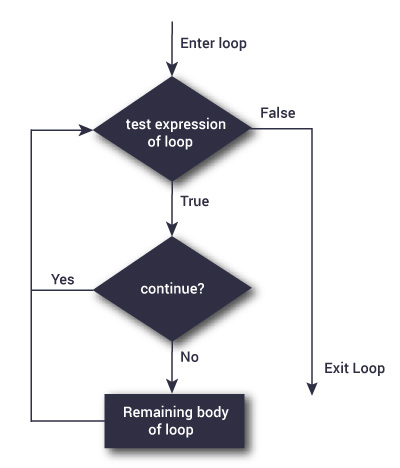
\includegraphics[width=0.4\linewidth]{img/continue}
	\caption{Mô tả cách thức hoạt động của từ khoá continue}
\end{figure}
\textbf{Ví dụ:} Tính căn bậc 2 của các phần tử trong dãy cho trước, bỏ qua các phần tử âm:\\
\rule{\linewidth}{0.2mm}\par
\begin{linenumbers}
	\texttt{\textcolor{red}{import} math}\par
	\smallskip
	\texttt{array = [1, 4, -5, 25, -8, 16]}\par
	\texttt{\textcolor{red}{for} i \textcolor{red}{in} array:}\par
	\qquad\texttt{\#skip element which is less than 0}\par
	\qquad\texttt{\textcolor{red}{if} i < 0:}\par
	\qquad\qquad\texttt{continue}\par
	\qquad\texttt{\textcolor{blue}{print}(math.sqrt(i))}\par
\end{linenumbers}
\rule{\linewidth}{0.2mm}\par
\noindent
\resetlinenumber
Kết quả cho ra ở Console:\\
\rule{\linewidth}{0.2mm}\par
\begin{linenumbers}
	\texttt{1.0}\par
	\texttt{2.0}\par
	\texttt{5.0}\par
	\texttt{4.0}\par
\end{linenumbers}
\rule{\linewidth}{0.2mm}\par
\resetlinenumber
\newpage
\subsubsection{Break}
Sử dụng từ khoá \texttt{break} khi người lập trình muốn dừng và thoát khỏi vòng lặp ngay lập tức.\par
\begin{figure}[h]
	\centering
	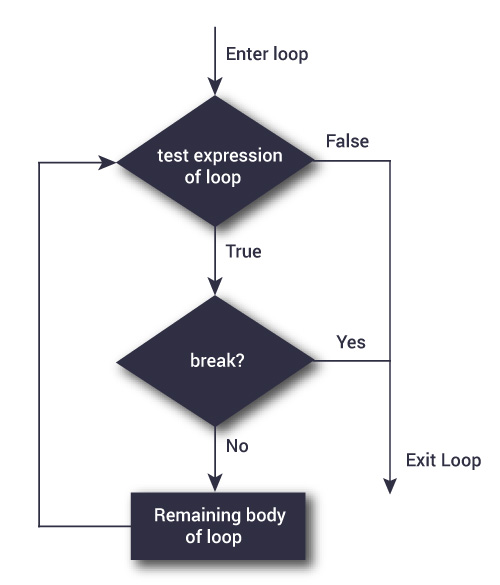
\includegraphics[width=0.4\linewidth]{img/break}
	\caption{Mô tả cách thức hoạt động của từ khoá break}
\end{figure}
\noindent
\textbf{Ví dụ:} Duyệt một chuỗi cho trước, lưu từng ký tự của chuỗi đó vào chuỗi mới, gặp kí tự 'E' thì ngừng lại:\\
\rule{\linewidth}{0.2mm}\par
\begin{linenumbers}
	\texttt{string = "contentE0xp"}\par
	\texttt{result = ""}\par
	\texttt{\textcolor{red}{for} i \textcolor{red}{in} string:}\par
	\qquad\texttt{\textcolor{red}{if} i == 'E':}\par
	\qquad\qquad\texttt{break}\par
	\qquad\texttt{result += i}\par
	\texttt{\textcolor{blue}{print}(result)}\par
\end{linenumbers}
\rule{\linewidth}{0.2mm}\par
\noindent
\resetlinenumber
Kết quả cho ra ở Console:\\
\rule{\linewidth}{0.2mm}\par
\begin{linenumbers}
	\texttt{content}\par
\end{linenumbers}
\rule{\linewidth}{0.2mm}\par
\resetlinenumber
\newpage
\subsubsection{Pass}
Khi người lập trình viết một vòng lặp hoặc một hàm, nhưng chưa có ý tưởng gì cho nó, thì có thể sử dụng từ khoá \texttt{pass} để thêm vào như là một câu lệnh giữ chỗ.\par
Nói một cách khác, \texttt{pass} là một lệnh trống, không làm gì cả. Python quy định các hàm và vòng lặp không được để trống. Vì thế, sử dụng từ khoá \texttt{pass} như là một câu lệnh để hợp thức hoá quy định trên.\par
Ví dụ về từ khoá \texttt{pass}:\\
\rule{\linewidth}{0.2mm}\par
\begin{linenumbers}
	\texttt{array = ['p', 'a', 's', 's']}\par
	\texttt{\textcolor{red}{for} i \textcolor{red}{in} array:}\par
	\qquad\texttt{pass}\par
	\texttt{\textcolor{blue}{print}("Pass successfully!")}\par
\end{linenumbers}
\rule{\linewidth}{0.2mm}\par
\noindent
\resetlinenumber
Kết quả cho ra ở Console:\\
\rule{\linewidth}{0.2mm}\par
\begin{linenumbers}
	\texttt{Pass successfully!}
\end{linenumbers}
\rule{\linewidth}{0.2mm}\par
\resetlinenumber
\newpage
	\section{Ngoại lệ và xử lý ngoại lệ}
\label{exception}
\subsection{Ngoại lệ là gì? Các loại ngoại lệ trong Python}
Ngoại lệ (exception) là lỗi xuất hiện làm dừng chương trình đang thực thi. Trong Python hỗ trợ các lập trình viên xử lý ngoại lệ để duy trì hoạt động cho chương trình.\par
Các Exception sẵn có của Python thông thường được bắt nguồn từ BaseException. Trong khi đó các exception của lập trình viên nên thừa kế từ lớp Exception hoặc từ các lớp con của nó. 
\begin{figure}[h]
	\centering
	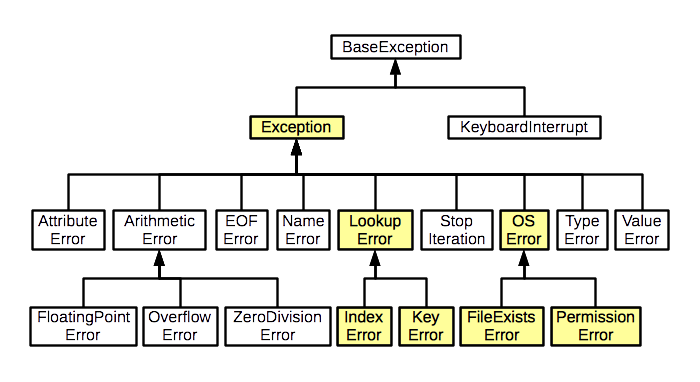
\includegraphics[width=0.7\linewidth]{img/exception}
	\caption{Sơ đồ mô tả các loại Exception trong Python}
\end{figure}
\newpage
\begin{table}[h]
	\centering
	\begin{tabular}{|l||p{12cm}|}
		\hline
		Tên ngoại lệ & Chú thích \\
		\hline
		\hline
		Exception & Đây là lớp cơ sở cho tất cả các exception, nó sẽ xuất hiện khi có bất cứ một lỗi nào xảy ra. \\
		\hline
		StopIteration & Xuất hiện khi phương thức next() của interator không trỏ đến một đối tượng nào.\\
		\hline
		SystemExit &	Xuất hiện khi dùng phương thức sys.exit().\\
		\hline
		ArithmeticError & Xuất hiện khi có lỗi tính toán giữa các số với nhau.\\
		\hline
		OverflowError &	Xuất hiện khi thực hiện tính toán và giá trị của nó vượt quá ngưỡng giới hạn cho phép của kiểu dữ liệu.\\
		\hline
		FloatingPointError &	Xuất hiện khi tính toán float thất bại.\\
		\hline
		ZeroDivisonError &	Xuất hiện khi thực hiện phép chia cho 0.\\
		\hline
		AssertionError &	Xuất hiện trong trường hợp lệnh assert thất bại.\\
		\hline
		AttributeError &	Xuất hiện khi không tồn tại thuộc tính này, hoặc thiếu tham số truyền vào nó.\\
		\hline
		EOFError &	Xuất hiện khi không có dữ liệu từ hàm input() hoặc cuối file.\\
		\hline
		ImportError &	Xuất hiện khi lệnh import thất bại.\\
		\hline
		KeyboardInterrupt &	Xuất hiện khi ngắt trình biên dịch.\\
		\hline
		LookupError &	Lớp cơ sở cho tất cả các lỗi về lookup.\\
		\hline
		IndexError &	Xuất hiện khi index không tồn tại trong list, string,...\\
		\hline
		KeyError &	Xuất hiện khi key không tồn tại trong dictionary.\\
		\hline
		NameError &	Xuất hiện khi một biến không tồn tại trong phạm vi bạn gọi nó.\\
		\hline
		EnvironmentError &	Xuất hiện khi có bất kỳ một lỗi nào ngoài phạm vi của Python.\\
		\hline
		IOError &	Xuất hiện khi xử dụng input/ output thất bại, hoặc  mở file không thành công.\\
		\hline
		OSError &	Xuất hiện khi có lỗi từ hệ điều hành.\\
		\hline
		SyntaxError &	Xuất hiện khi chương trình có lỗi cú pháp.\\
		\hline
		IndentationError &	Xuất hiện khi bạn thụt dòng không đúng.\\
		\hline
		SystemError &	Xuất hiện khi trình biên dịch có vấn đề nhưng mà nó lại không tự động exit.\\
		\hline
		SystemExit &	Xuất hiện khi trình biên dịch được thoát bởi sys.exit().\\
		\hline
		TypeError &	Xuất hiện khi thực thi toán tử hoặc hàm mà kiểu dữ liệu bị sai so với kiểu dữ liệu đã định nghĩa ban đầu.\\
		\hline
		ValueError &	Xuất hiện khi chúng ta build 1 function mà kiểu dữ liệu đúng nhưng khi chúng ta thiết lập ở tham số là khác so với khi truyền vào.\\
		\hline
		RuntimeError &	Xuất hiện khi lỗi được sinh ra không thuộc một danh mục nào.\\
		\hline
		NotImplementedError &	Xuất hiện khi một phương thức trừu tượng cần được thực hiện trong lớp kế thừa chứ không phải là lớp thực thi.\\
		\hline
		UnboundLocalError &	Xuất hiện khi chúng ta cố tình truy cập vào một biến trong hàm hoặc phương thức, nhưng không thiết lập giá trị cho nó.\\
		\hline
	\end{tabular}
	\caption{Các ngoại lệ trong Python}
\end{table}
\newpage
\textbf{Ví dụ:} Duyệt qua một list số nguyên, in ra giá trị nghịch đảo của từng phần tử trong list:\\
\rule{\linewidth}{0.2mm}\par
\begin{linenumbers}
	\texttt{list = [4, 5, 0, 7]}\par
	\texttt{\textcolor{red}{for} i \textcolor{red}{in} list:}\par
	\qquad\texttt{\textcolor{blue}{print}(1 / i)}\par
\end{linenumbers}
\rule{\linewidth}{0.2mm}\par
\noindent
\resetlinenumber
Kết quả cho ra ở Console:\\
\rule{\linewidth}{0.2mm}\par
\begin{linenumbers}
	\texttt{0.25}\par
	\texttt{0.2}\par
	\texttt{Traceback (most recent call last):}\par
	\texttt{File "Exception.py", line 3, in <module>}\par
	\qquad\texttt{print(1/i)}\par
	\texttt{ZeroDivisionError: division by zero}
\end{linenumbers}
\rule{\linewidth}{0.2mm}\par
\resetlinenumber
Khi duyệt đến phần tử \texttt{array[2] = 0}, việc tính toán giá trị $\frac{1}{i}$ gặp lỗi chia cho 0. Do đó, chương~trình dừng lại ngay lập tức và in lỗi ra ngoài Console, không tiếp tục duyệt các phần tử còn lại của list.
\newpage
\textbf{Ví dụ:} Duyệt qua một list chứa nhiều kiểu dữ liệu, in ra tổng giá trị các số trong list:\\
\rule{\linewidth}{0.2mm}\par
\begin{linenumbers}
	\texttt{list = [1, 2.3, 7.6, "Ex"]}\par
	\texttt{sum = 0.0}\par
	\texttt{\textcolor{red}{for} i \textcolor{red}{in} list:}\par
	\qquad\texttt{sum += i}\par
	\texttt{\textcolor{blue}{print}(sum)}\par
\end{linenumbers}
\rule{\linewidth}{0.2mm}\par
\noindent
\resetlinenumber
Kết quả cho ra ở Console:\\
\rule{\linewidth}{0.2mm}\par
\begin{linenumbers}
	\texttt{Traceback (most recent call last):}\par
	\texttt{File "Exception.py", line 4, in <module>}\par
	\qquad\texttt{sum += i}\par
	\texttt{TypeError: unsupported operand type(s) for +=: 'float' and 'str'}
\end{linenumbers}
\rule{\linewidth}{0.2mm}\par
Khi duyệt đến phần tử \texttt{"Ex"}, Python không thể chuyển kiểu dữ liệu chuỗi sang kiểu số và cộng vào biến \texttt{sum}, từ đó xảy ra lỗi \texttt{TypeError}.
\resetlinenumber
\newpage
\subsection{Xử lý ngoại lệ với try - except - finally}
Ta có thể xử lý ngoại lệ bằng cách đặt phần code có khả năng xảy ra lỗi vào trong câu lệnh \texttt{try - except}. Lập trình viên có thể in các mô tả về ngoại lệ xảy ra trong đoạn code ra màn hình, hoặc có thể bỏ qua chúng.\par
Cấu trúc câu lệnh try - catch - finally:\par
\rule{\linewidth}{0.2mm}\par
\texttt{try:}\par
\qquad\texttt{\# code}\par
\texttt{except <exception\_name> as <variable\_name>:}\par
\qquad\texttt{\# handle code}\par
\texttt{[finally:}\par
\qquad\texttt{\# code]}\par
\rule{\linewidth}{0.2mm}\par
Cách thức hoạt động của try - catch - finally diễn ra như sau: Khi các câu lệnh trong try được phát hiện xảy ra ngoại lệ, chương trình sẽ chuyển xuống phần except và thực hiện các câu lệnh xử lý ngoại lệ trong nó. Sau khi xử lý xong ngoại lệ, tiếp tục thực hiện các câu lệnh trong finally (nếu có). Trường hợp trong try không có ngoại lệ, chương trình vẫn thực hiện các câu lệnh trong finally.\par
Khác với Java, lập trình viên có thể khai báo nhiều ngoại lệ có thể xảy ra trong chương trình mà không cần phải tuân thủ quy tắc từ cụ thể đến chung nhất. Python sẽ tự tìm kiếm một exception phù hợp trong các exception mà lập trình viên đã khai báo mà không quan tâm đến các ngoại lệ còn lại. Thứ tự xét các exception là từ trên xuống.
\newpage
\textbf{Ví dụ:} In các giá trị căn bậc 2 của từng phần tử trong một list, bỏ qua các giá trị âm:\\
\rule{\linewidth}{0.2mm}\par
\begin{linenumbers}
	\texttt{\textcolor{red}{from} math \textcolor{red}{import} sqrt}\par
	\medskip
	\texttt{list = [4, 16, -7, 25]}\par
	\texttt{\textcolor{red}{for} i \textcolor{red}{in} list:}\par
	\qquad\texttt{\textcolor{red}{try:}}\par
	\qquad\qquad\texttt{\textcolor{blue}{print}(sqrt(i))}\par
	\qquad\texttt{\textcolor{red}{except} Exception \textcolor{red}{as} e:}\par
	\qquad\qquad\texttt{\textcolor{red}{pass} \# skip if it's a negative number}\par
	\qquad\texttt{\textcolor{red}{finally}:}\par
	\qquad\qquad\texttt{\textcolor{blue}{print}("Done!")}\par
\end{linenumbers}
\rule{\linewidth}{0.2mm}\par
\noindent
\resetlinenumber
Kết quả cho ra ở Console:\\
\rule{\linewidth}{0.2mm}\par
\begin{linenumbers}
	\texttt{2.0}\par
	\texttt{Done!}\par
	\texttt{4.0}\par
	\texttt{Done!}\par
	\texttt{Done!}\par
	\texttt{5.0}\par
	\texttt{Done!}\par
\end{linenumbers}
\rule{\linewidth}{0.2mm}\par
\resetlinenumber
Khi xét đến phần tử -7, do không thể lấy căn bậc 2 của một số âm nên chương trình xét đoạn lệnh trong phần \texttt{except}. Từ khoá \texttt{pass} không thực hiện câu lệnh nào cả, chương trình chạy đến phần \texttt{finally}, in dòng chữ \texttt{"Done!"} ra ngoài màn hình rồi tiếp tục xét các giá trị khác trong list.
\newpage
\textbf{Ví dụ:} Duyệt và in ra các phần tử trong một list bằng chỉ số:\\
\rule{\linewidth}{0.2mm}\par
\begin{linenumbers}
	\texttt{ls = [1, 2, 0.2, 3]}\par
	\texttt{\textcolor{red}{for} i \textcolor{red}{in} range(len(ls) + 1):}\par
	\qquad\texttt{\textcolor{red}{try:}}\par
	\qquad\qquad\texttt{\textcolor{blue}{print}(ls[i])}\par
	\qquad\texttt{\textcolor{red}{except} ZeroDivisionError \textcolor{red}{as} e:}\par
	\qquad\qquad\texttt{\textcolor{blue}{print}(e)}\par
	\qquad\texttt{\textcolor{red}{except} LookupError \textcolor{red}{as} ex:}\par
	\qquad\qquad\texttt{\textcolor{blue}{print}(ex.\_\_doc\_\_)  \# output: Sequence index out of range.}\par
	\qquad\texttt{\textcolor{red}{except} IndexError \textcolor{red}{as} exc:}\par
	\qquad\qquad\texttt{\textcolor{blue}{print}(ex)  \# output: list index out of range.}\par
\end{linenumbers}
\rule{\linewidth}{0.2mm}\par
\noindent
\resetlinenumber
Kết quả cho ra ở Console:\\
\rule{\linewidth}{0.2mm}\par
\begin{linenumbers}
	\texttt{1}\par
	\texttt{2}\par
	\texttt{0.2}\par
	\texttt{3}\par
	\texttt{Sequence index out of range.}\par
\end{linenumbers}
\rule{\linewidth}{0.2mm}\par
\resetlinenumber
Do chỉ có 4 phần tử trong list \texttt{ls} nên các phần tử trong list được đánh số từ 0 đến 3. Hàm \texttt{range(len(ls)~+~1)} trả về một mảng số nguyên \texttt{[0, 1, 2, 3, 4]}. Khi duyệt đến phần tử có chỉ số 4 trong list, chương trình phát sinh ra lỗi và tìm đến exception phù hợp đầu tiên mà người lập trình đã khai báo là \texttt{LookupError} rồi thực hiện câu lệnh \texttt{print(ex.\_\_doc\_\_)}, bỏ qua exception \texttt{IndexError} mặc dù ngoại lệ này là cụ thể nhất cho lỗi phát sinh.
\newpage
\subsection{Ngoại lệ do người dùng tự định nghĩa}
Ngoài các ngoại lệ đã mô tả ở phần trên, lập trình viên có thể tự định nghĩa một ngoại lệ riêng sao cho phù hợp với từng chương trình cụ thể bằng từ khoá \texttt{raise}.\par
\textbf{Ví dụ:} Chương trình tính tiền thuê phòng khách sạn, mỗi giờ là \$5, số giờ không được dưới 1 và trên 12.:\\
\rule{\linewidth}{0.2mm}\par
\begin{linenumbers}
	\texttt{hour = [1, 5, 7, 0.5, 11]}\par
	\texttt{\textcolor{red}{for} i \textcolor{red}{in} hour:}\par
	\qquad\texttt{\textcolor{red}{if} i < 1 \textcolor{red}{or} i > 12:}\par
	\qquad\qquad\texttt{\textcolor{red}{raise} Exception("Hour must be greater than 1 and less than 12")}\par
	\qquad\texttt{\textcolor{blue}{print}("Price: \%d\$" \% (i * 5))}\par
\end{linenumbers}
\rule{\linewidth}{0.2mm}\par
\noindent
\resetlinenumber
Kết quả cho ra ở Console:\\
\rule{\linewidth}{0.2mm}\par
\begin{linenumbers}
	\texttt{Traceback (most recent call last):}\par
	\texttt{File "Exception.py", line 4, in <module>}\par
	\qquad\texttt{raise Exception("Hour must be greater than 1 and less than 12")}\par
	\texttt{Exception: Hour must be greater than 1 and less than 12}\par
	\texttt{Price: 5\$}\par
	\texttt{Price: 25\$}\par
	\texttt{Price: 35\$}\par
\end{linenumbers}
\rule{\linewidth}{0.2mm}\par
\resetlinenumber
\end{document}